\paragraph{QuizziPedia::Front-End::Controllers::SearchController}
\begin{figure} [ht]
	\centering
	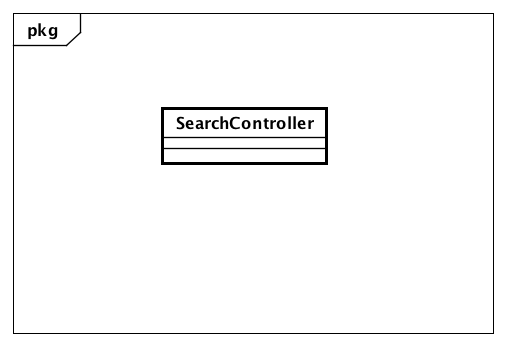
\includegraphics[scale=0.5]{UML/Classi/Front-End/QuizziPedia_Front-end_Controller_SearchController.png}
	\caption{QuizziPedia::Front-End::Controllers::SearchController}
\end{figure} \FloatBarrier
\begin{itemize}
	\item \textbf{Descrizione}: questa classe permette di gestire la ricerca di questionari e utenti all'interno dell'applicazione;
	\item \textbf{Utilizzo}: fornisce all'utente le funzionalità di ricerca per utenti e questionari;
	\item \textbf{Relazione con altre classi}:
	\begin{itemize}
		\item \textbf{IN \texttt{ResultsModelView}}: classe di tipo \textit{modelview\ped{G}} la cui istanziazione è contenuta all'interno della variabile di ambiente \$scope di \textit{Angular\ped{G}}. All'interno di essa sono presenti le variabili e i metodi necessari per il \textit{Two-Way Data-Binding\ped{G}} tra la \textit{view\ped{G}} \texttt{ResultsView}, la \textit{directive\ped{G}} \texttt{SearchDirective} e il \textit{controller\ped{G}} \texttt{ResultsController};
		\item \textbf{IN \texttt{SearchService}}: questa classe permette di eseguire una ricerca tra i questionari e gli utenti presenti ritornando un Object contenente i risultati di tale operazione;
		\item \textbf{IN \texttt{QuizService}}: questa classe permette di ottenere i dati di un quiz tramite delle parole chiave inserite dall'utente nella barra di ricerca. Permette inoltre di iscriversi ad un questionario.
	\end{itemize}
	\item \textbf{Attributi}:
	\begin{itemize}
		\item \texttt{-} \texttt{\$scope: \$scope} \\
		Campo dati contenente un riferimento all'oggetto \$scope creato da \textit{Angular\ped{G}}, viene utilizzato come mezzo di comunicazione tra il \textit{controller\ped{G}} e la \textit{view\ped{G}}. Contiene gli oggetti che definiscono il \textit{model\ped{G}} dell'applicazione;
		\item \texttt{-} \texttt{\$location: \$location} \\
		Campo dati contenente un riferimento al servizio creato da \textit{Angular\ped{G}} che permette di accedere alla barra degli indirizzi del \textit{browser\ped{G}}, i cambiamenti all'URL nella barra degli indirizzi si riflettono in questo oggetto e viceversa;
		\\item \texttt{-} \texttt{\$mdDialog: \$mdDialog} \\
		Campo dati contenente un riferimento al servizio della libreria \textit{Material for Angular\ped{G}} che permette di creare delle componenti a pop-up;
		\item \texttt{-} \texttt{\$routeParams: \$routeParams} \\
		Campo dati contente un riferimento al servizio creato da \textit{Angular\ped{G}} che permette di accedere alla barra degli indirizzi e recuperare i parametri passati; 
		\item \texttt{-} \texttt{SearchService: SearchService} \\
		Campo dati contenente un riferimento al servizio che si occupa della gestione delle informazioni legate alla ricerca. Viene utilizzato il metodo \texttt{search} di \texttt{SearchService} a cui viene passato come parametro la stringa di ricerca;
		\item \texttt{-} \texttt{QuizService: QuizService} \\
		Campo dati contenente un riferimento al servizio che si occupa della gestione delle informazioni legate ai questionari. Viene utilizzato il metodo \texttt{subscribeQuestionnaire} di \texttt{QuizService} per iscrivere un utente ad un questionario;
		\item \texttt{+} \texttt{result: ResultsModelView} \\
		Oggetto di tipo \texttt{ResultsModelView}. All'interno di esso sono presenti le variabili e i metodi necessari per il \textit{Two-Way Data-Binding\ped{G}} tra la \textit{view\ped{G}} \texttt{ResultView} e il \textit{controller\ped{G}} \texttt{SearchController}.
	\end{itemize}
	\item \textbf{Metodi}:
	\begin{itemize}
		\item \texttt{+} \texttt{SearchController(\$scope: \$scope, \$location: \$location, \$mdDialog: \$mdDialog, \$routeParams: \$routeParams, SearchService: SearchService, QuizService: QuizService)} \\
		Metodo costruttore della classe. Viene eseguita la ricerca per poter poi popolare il campo dati \texttt{result}. \\
		\textbf{Parametri}:
		\begin{itemize}
			\item \texttt{\$scope: \$scope} \\
			Parametro contenente un riferimento all'oggetto \$scope creato da \textit{Angular\ped{G}}. Viene utilizzato come mezzo di comunicazione tra il \textit{controller\ped{G}} e la \textit{view\ped{G}}. Contiene gli oggetti che definiscono il \textit{viewmodel\ped{G}} e il \textit{model\ped{G}} dell'applicazione;
			\item \texttt{\$location: \$location} \\
			Parametro contenente un riferimento al servizio creato da \textit{Angular\ped{G}} che permette di accedere alla barra degli indirizzi del \textit{browser\ped{G}}, i cambiamenti all'URL nella barra degli indirizzi si riflettono in questo oggetto e viceversa;
			\item \texttt{\$mdDialog: \$mdDialog} \\
			Parametro contenente un riferimento al servizio della libreria \textit{Material for Angular\ped{G}} che permette di creare delle componenti a pop-up;
			\item \texttt{\$routeParams: \$routeParams} \\
			Parametro contente un riferimento al servizio creato da \textit{Angular\ped{G}} che permette di accedere alla barra degli indirizzi e recuperare i parametri passati;
			\item \texttt{SearchService: SearchService} \\
			Parametro contenente un riferimento al servizio che si occupa della gestione delle informazioni legate alla ricerca. Viene utilizzato il metodo \texttt{search} di \texttt{SearchService} a cui viene passato come parametro la stringa di ricerca;
			\item \texttt{QuizService: QuizService} \\
			Parametro contenente un riferimento al servizio che si occupa della gestione delle informazioni legate ai questionari. Viene utilizzato il metodo \texttt{subscribeQuestionnaire} di \texttt{QuizService} per iscrivere un utente ad un questionario.
		\end{itemize} 
		\item \texttt{-} \texttt{getSearch(stringSearch: String): SearchModelView} \\
		Metodo che esegue la ricerca utilizzando un metodo fornito dalla classe \texttt{SearchService}. \\
		\textbf{Parametri}:
		\begin{itemize}
			\item \texttt{stringSearch: String} \\
			Parametro contenente la stringa sulla quale si deve basare la ricerca.
		\end{itemize} 
		\item \texttt{+} \texttt{goToUser(username: String): void} \\
		Metodo che gestisce l'evento click sul bottone per visualizzare il profilo dell'utente selezionato. Effettua il redirect alla pagina dell'utente.\\
		\textbf{Parametri}:
		\begin{itemize}
			\item \texttt{username: String} \\
			Parametro contenente l'username dell'utente di cui si vuole visualizzare il profilo.
		\end{itemize} 
		\item \texttt{+} \texttt{registrationToQuiz(idQuiz: String): void} \\
		Metodo che gestisce l'evento click sul pulsante di registrazione al questionario.\\
		\textbf{Parametri}:
		\begin{itemize}
			\item \texttt{idQuiz: String} \\
			Parametro contenente l'id del questionario di cui si vuole effettuare l'iscrizione.
		\end{itemize} 
		\item \texttt{+} \texttt{goToResultsPage(stringSearch: String): void} \\
		Metodo che gestisce l'evento click sul pulsante per effettuare una ricerca.\\
		\textbf{Parametri}:
		\begin{itemize}
			\item \texttt{stringSearch: String} \\
			Parametro contenente la stringa sulla quale si deve basare la ricerca.
		\end{itemize} 
	\end{itemize}
\end{itemize}

